\documentclass[10pt,xcolor=table]{beamer}
 
% \usepackage[utf8]{inputenc}
% \usepackage[T1]{fontenc}
\usepackage[table]{xcolor}    % loads also »colortbl« 
%  \usepackage{enumitem}
\usepackage{ucltemplate}
\usepackage{color}
\usepackage{amsmath,amssymb,calc,ifthen,capt-of}

% \definecolor{parCol}{rgb}{0.1, 0.1, 1}
% \definecolor{stCol}{rgb}{0.1, 0.6, 0.1}
% \definecolor{bothCol}{rgb}{0, 0.5, 0.5}

\definecolor{parCol}{rgb}{0, 0, 0}
\definecolor{stCol}{rgb}{0, 0, 0}
\definecolor{bothCol}{rgb}{0, 0, 0}



 
%Information to be included in the title page:
\title{A mixed-effects model with time reparametrization for longitudinal univariate manifold-valued data}
\author{Schiratti J. B. et al.}
\institute{IPMI 2015}
% \date{15 November 2016}

% % logo of my university
% \titlegraphic{
\includegraphics[height=1.0cm]{epsrc_logo.jpg}\hspace*{1.75cm}~%
%    
\includegraphics[height=1.5cm]{NEWpond2017b.png} \hspace*{1.75cm}~ 
%    
\includegraphics[height=1.0cm]{CDTlogo.png} 
% }
 
 
\setbeamersize{text margin left=15pt,text margin right=15pt,text margin bottom=15pt}


\begin{document}
 
\frame{\titlepage}
 
\setbeamerfont{frametitle}{size=\large}


\begin{frame}
\frametitle{Overview - Disease Progression Models}

Aims: 
\begin{itemize}
  \item understand the progression of the disease
  \item accurately stage subjects in clinical trials
  \item prognosis
\end{itemize}

\begin{figure}
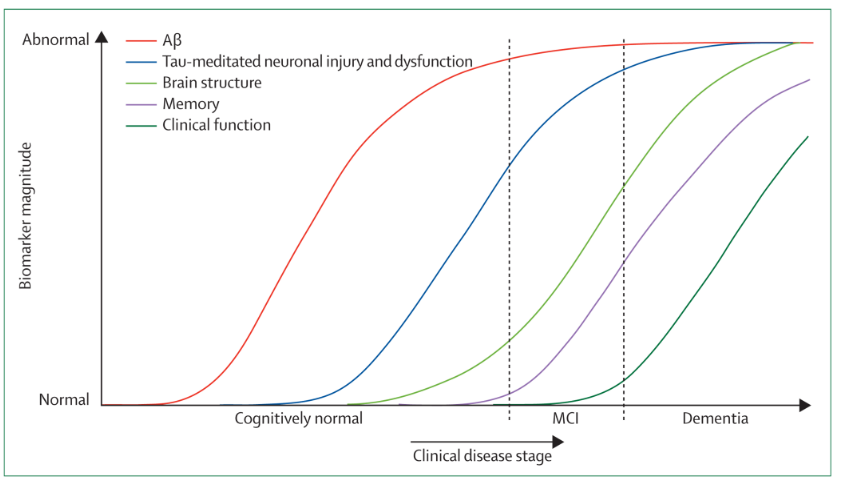
\includegraphics[scale=0.25]{jack_curves.png}
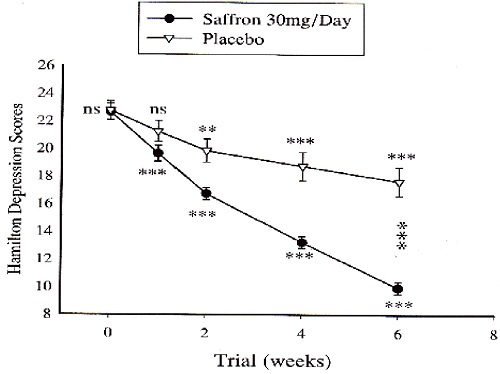
\includegraphics[scale=1]{drug_progression.jpg}
\end{figure}

\end{frame}

\begin{frame}
\frametitle{Timeline of disease progression models}

\newcommand{\colWidth}{2.5}

\begin{table}
\scriptsize

\begin{tabular}{p{3.5 cm} | p{2 cm} | p{\colWidth cm} | p{\colWidth cm}}
 Model & Trajectory shape & Subject staging & Main limitation \\
 \hline
 Comparison of symptomatic stages & not modelled at all & very coarse & biased categories\\
 Event-based Model & step-functions & discreete stages & no notion of time\\
 Differential Equation Models & non-parametric & both onset and speed & trajectories not aligned\\
 Disease Progression Score & sigmoids & both onset and speed & sigmoidal assumption\\
 Self-modelling regression & non-parametric & both onset and speed & -\\
 Manifold Model & sigmoids & both onset and speed & sigmoids have the same shape\\
\end{tabular}
\end{table}


% \begin{enumerate}
%  \item Comparison of symptomatic stages:e.g. "healthy", "mild", "moderate", "severe"
%  \item Event-based Model: assumes trajectories are step-functions + no notion of time between events
%  \item Differential Equation Models: can build non-parametric trajectories but no temporal alignment
%  \item Disease Progression Score: sigmoid trajectories + temporal alignment, subjects
% \end{enumerate}


\end{frame}

\begin{frame}
\frametitle{What is a manifold}

\begin{itemize}
 \item An N-dimensional space that generalises the Euclidean space
 \item Equipped with an inner product and distance metric
  
\end{itemize}

%TODO picture with image manifolds

\end{frame}


\begin{frame}
\frametitle{The model}

\begin{itemize}

 \item The model is a non-linear mixed effects model placed in a Riemannian manifold setting
  \item Each subject $i$ has an associated:
  \begin{itemize}
  \item time shift $\tau_i$
  \item progression speed $\alpha_i$
  \end{itemize}
  \item Fixed effects are:
  \begin{itemize}
  \item time shift $t_0$
  \item progression speed $v_0$
  \item observation point on the manifold $t_0$
  \end{itemize}
  \item The biomarker trajectory $\gamma_{p_0,t_0,v_0}$
%   \item The measurement for subject $i$ at visit $j$ is $y_{i,j}$ 


\end{itemize}


\begin{equation}
  y_{i,j} = \gamma_{p_0,t_0,v_0}(\alpha_iv_0(t_{i,j}-t_0-\tau_i))+\epsilon_{i,j} 
\end{equation}
where
\begin{equation}
\label{eq:manifold2}
\begin{cases}
  \alpha_i = exp(\nu_i)\\
  \nu_i \sim \bigotimes_{i=1}^p N(0, \sigma_{\nu}^2)\\  
  \tau_i \sim \bigotimes_{i=1}^p N(0, \sigma_{\tau}^2)\\  
  \epsilon_{i,j} \sim \bigotimes_{i,j} N(0, \sigma^2)\\  
\end{cases}
\end{equation}

\end{frame}

% \begin{frame}
% \frametitle{Some intuition}
% 
% \begin{figure}
% 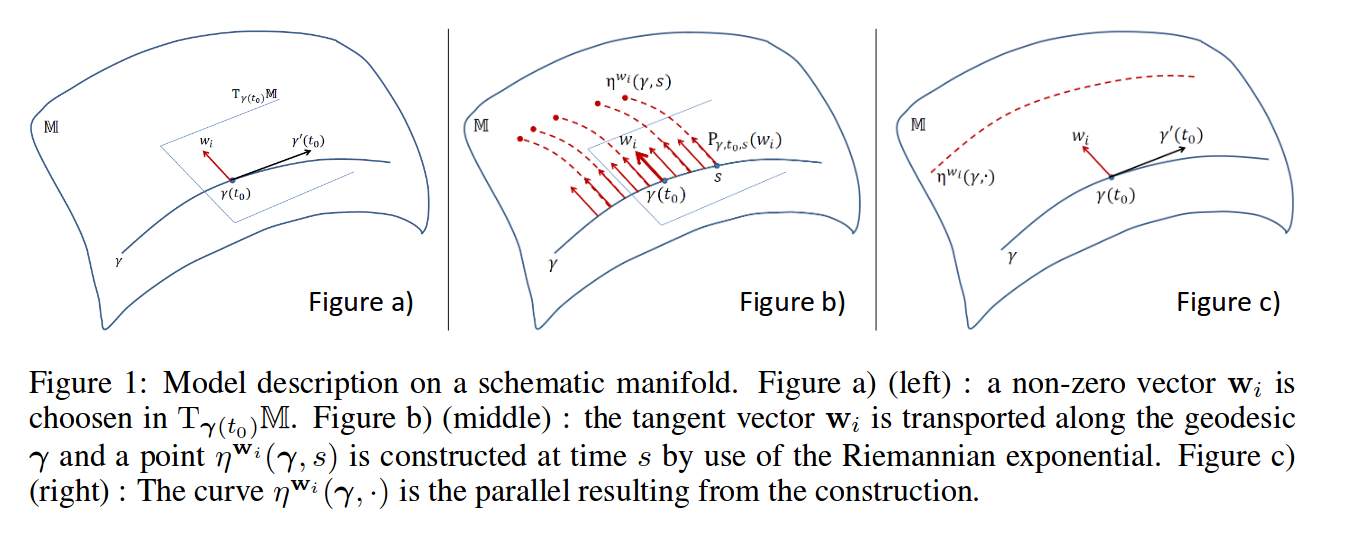
\includegraphics[scale=0.25]{manifold_schiratti_nips.png}
% \end{figure}
% 
% \end{frame}

\begin{frame}
\frametitle{Results - time shifts}

\begin{figure}
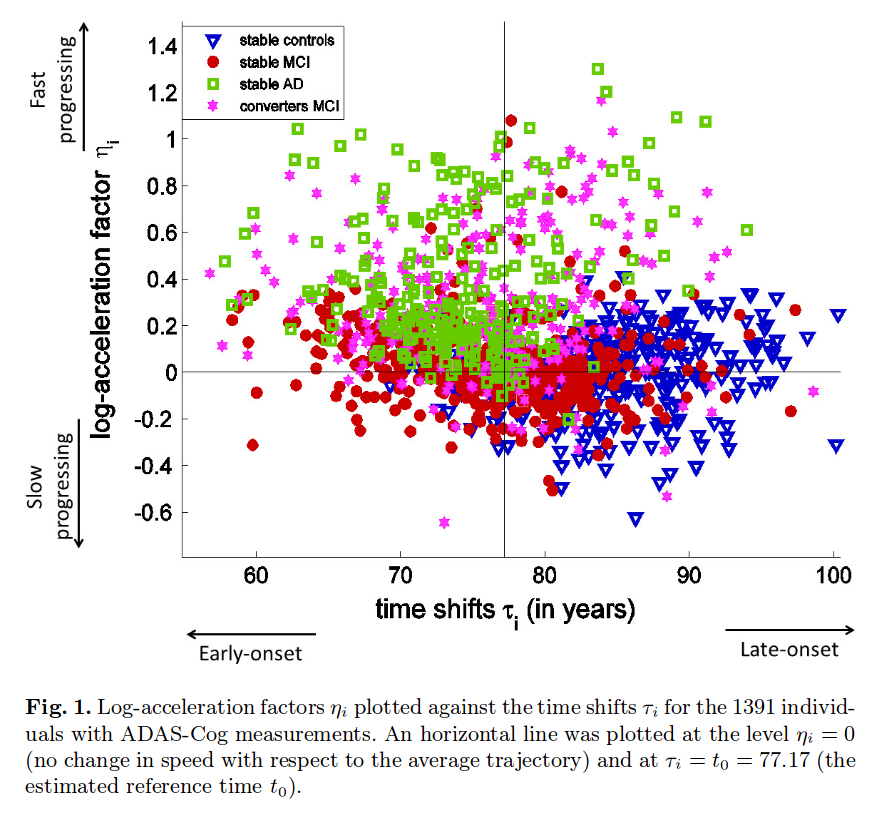
\includegraphics[scale=0.27]{res_fig1.png}
\end{figure}

\end{frame}

\begin{frame}
\frametitle{Results - AD vs stable controls}

\begin{figure}
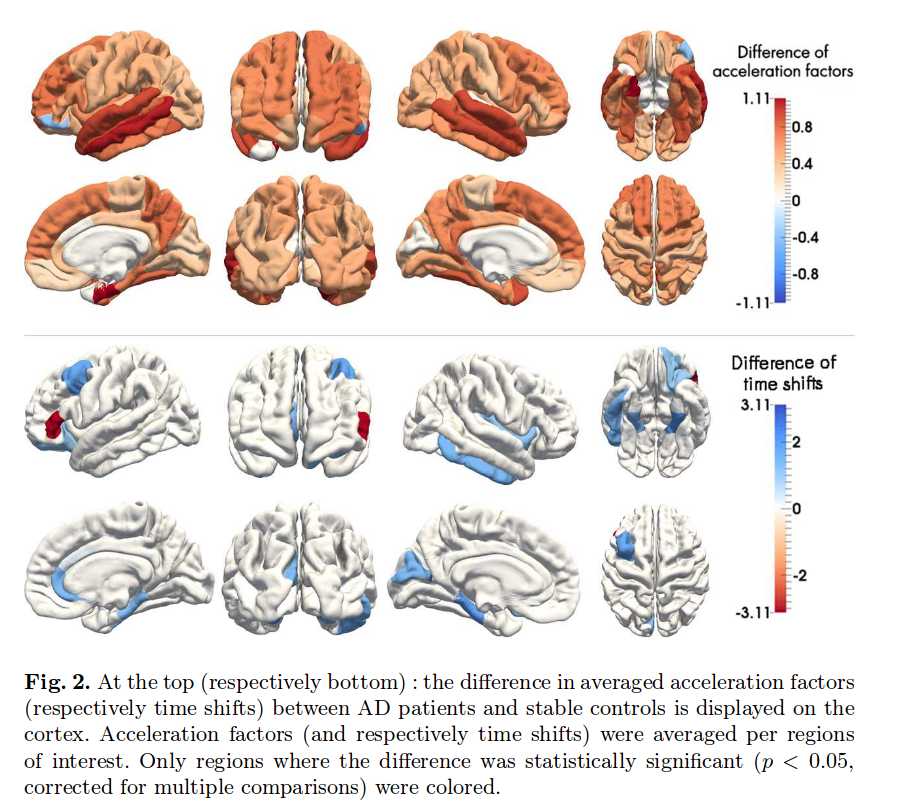
\includegraphics[scale=0.27]{res_fig2.png}
\end{figure}

\end{frame}

\begin{frame}
\frametitle{Results - MCI converters vs MCI stable}

\begin{figure}
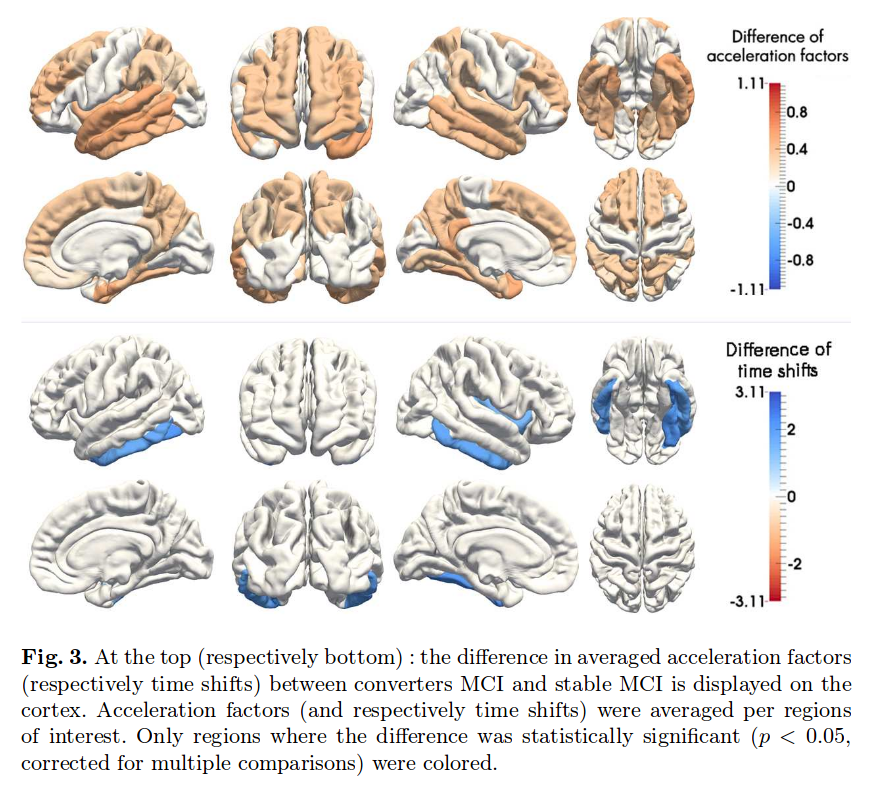
\includegraphics[scale=0.27]{res_fig3.png}
\end{figure}

\end{frame}


\fontsize{6pt}{7.2}\selectfont
\rowcolors{2}{gray!25}{white}

% \begin{frame}
% \frametitle{Validation methods for disease progression models}
% 
% \begin{tabular}{p{3.3cm} p{3.3cm} p{3.3cm}}
%  Method & Pros & Cons\\
%  \hline
%  AIC/BIC & no extra data required & \\
%  Staging consistency & &\\
%  Elapsed time prediction & &\\ 
%  Diagnosis prediction and differential diagnosis & & diagnosis not precise, required post-mortem confirmed data\\
%  Correlation of stages with clinical markers & & relationship not linear\\
%  Simulations & ground truth available & simulated data might not reflect actual data\\
%  Prediction of leave-out biomarkers & & \\
%  Resampling methods & can also be used to test accuracy of model parameters & computationally intensive\\
%  Reproducibility across models and datasets & & requires different datasets\\
% \end{tabular}
% 
% \end{frame}


 
\end{document}

